\documentclass[12pt]{beamer}\usepackage[]{graphicx}\usepackage[]{color}
%% maxwidth is the original width if it is less than linewidth
%% otherwise use linewidth (to make sure the graphics do not exceed the margin)
\makeatletter
\def\maxwidth{ %
  \ifdim\Gin@nat@width>\linewidth
    \linewidth
  \else
    \Gin@nat@width
  \fi
}
\makeatother

\definecolor{fgcolor}{rgb}{0.345, 0.345, 0.345}
\newcommand{\hlnum}[1]{\textcolor[rgb]{0.686,0.059,0.569}{#1}}%
\newcommand{\hlstr}[1]{\textcolor[rgb]{0.192,0.494,0.8}{#1}}%
\newcommand{\hlcom}[1]{\textcolor[rgb]{0.678,0.584,0.686}{\textit{#1}}}%
\newcommand{\hlopt}[1]{\textcolor[rgb]{0,0,0}{#1}}%
\newcommand{\hlstd}[1]{\textcolor[rgb]{0.345,0.345,0.345}{#1}}%
\newcommand{\hlkwa}[1]{\textcolor[rgb]{0.161,0.373,0.58}{\textbf{#1}}}%
\newcommand{\hlkwb}[1]{\textcolor[rgb]{0.69,0.353,0.396}{#1}}%
\newcommand{\hlkwc}[1]{\textcolor[rgb]{0.333,0.667,0.333}{#1}}%
\newcommand{\hlkwd}[1]{\textcolor[rgb]{0.737,0.353,0.396}{\textbf{#1}}}%
\let\hlipl\hlkwb

\usepackage{framed}
\makeatletter
\newenvironment{kframe}{%
 \def\at@end@of@kframe{}%
 \ifinner\ifhmode%
  \def\at@end@of@kframe{\end{minipage}}%
  \begin{minipage}{\columnwidth}%
 \fi\fi%
 \def\FrameCommand##1{\hskip\@totalleftmargin \hskip-\fboxsep
 \colorbox{shadecolor}{##1}\hskip-\fboxsep
     % There is no \\@totalrightmargin, so:
     \hskip-\linewidth \hskip-\@totalleftmargin \hskip\columnwidth}%
 \MakeFramed {\advance\hsize-\width
   \@totalleftmargin\z@ \linewidth\hsize
   \@setminipage}}%
 {\par\unskip\endMakeFramed%
 \at@end@of@kframe}
\makeatother

\definecolor{shadecolor}{rgb}{.97, .97, .97}
\definecolor{messagecolor}{rgb}{0, 0, 0}
\definecolor{warningcolor}{rgb}{1, 0, 1}
\definecolor{errorcolor}{rgb}{1, 0, 0}
\newenvironment{knitrout}{}{} % an empty environment to be redefined in TeX

\usepackage{alltt}
\usepackage{tikz}

% make it pretty
% get rid of junk
\usetheme{default}
\usefonttheme[onlymath]{serif}
\beamertemplatenavigationsymbolsempty

% define a bunch of colors
\definecolor{offwhite}{RGB}{255,250,240}
\definecolor{gray}{RGB}{155,155,155}
\definecolor{foreground}{RGB}{80,80,80}
\definecolor{background}{RGB}{255,255,255}
%\definecolor{title}{RGB}{255,199,0}
\definecolor{title}{RGB}{89,132,212}
%\definecolor{subtitle}{RGB}{89,132,212}
\definecolor{subtitle}{RGB}{255,199,0}
\definecolor{hilit}{RGB}{248,117,79}
\definecolor{vhilit}{RGB}{255,111,207}
\definecolor{lolit}{RGB}{200,200,200}
\definecolor{lit}{RGB}{255,199,0}
\definecolor{mdlit}{RGB}{89,132,212}
\definecolor{link}{RGB}{248,117,79}

% a few color macros
\newcommand{\hilit}{\color{hilit}}
\newcommand{\vhilit}{\color{vhilit}}
\newcommand{\lit}{\color{lit}}
\newcommand{\mdlit}{\color{mdlit}}
\newcommand{\lolit}{\color{lolit}}

% use those colors
\setbeamercolor{titlelike}{fg=title}
\setbeamercolor{subtitle}{fg=subtitle}
\setbeamercolor{frametitle}{fg=gray}
%\setbeamercolor{structure}{fg=subtitle}
\setbeamercolor{structure}{fg=title}
\setbeamercolor{institute}{fg=lolit}
\setbeamercolor{normal text}{fg=foreground,bg=background}
\setbeamertemplate{itemize subitem}{{\textendash}}
\setbeamerfont{itemize/enumerate subbody}{size=\small}
\setbeamerfont{itemize/enumerate subitem}{size=\small}

% center title of slides
\setbeamertemplate{blocks}[rounded]
\setbeamertemplate{frametitle}[default][center]

% page number
\setbeamerfont{page number in foot}{size=\footnotesize}
\setbeamertemplate{footline}[frame number]

% default link color
\hypersetup{colorlinks, urlcolor={link}}

% a few macros
\newcommand{\code}[1]{\texttt{#1}}
\newcommand{\hicode}[1]{{\hilit \texttt{#1}}}
\newcommand{\locode}[1]{{\lolit \texttt{#1}}}
\newcommand{\bb}[1]{\begin{block}{#1}}
\newcommand{\eb}{\end{block}}
\newcommand{\bi}{\begin{itemize}}
\newcommand{\bbi}{\vspace{4pt} \begin{itemize} \itemsep8pt}
\newcommand{\ei}{\end{itemize}}
\newcommand{\bv}{\begin{verbatim}}
\newcommand{\ev}{\end{verbatim}}
\newcommand{\ig}{\includegraphics}
\newcommand{\subt}[1]{{\footnotesize \color{subtitle} {#1}}}
\newcommand{\ttsm}{\tt \small}
\newcommand{\ttfn}{\tt \footnotesize}
\newcommand{\figh}[2]{\centerline{\includegraphics[height=#2\textheight]{#1}}}
\newcommand{\figw}[2]{\centerline{\includegraphics[width=#2\textwidth]{#1}}}



%------------------------------------------------

\title{Entertainment}
\subtitle{Intro to Data Visualization}
\author{\href{http://www.gastonsanchez.com}{Gaston Sanchez}}
\institute{\href{https://creativecommons.org/licenses/by-sa/4.0/}{\tt \scriptsize \color{foreground} CC BY-SA 4.0}}
\date{}
\IfFileExists{upquote.sty}{\usepackage{upquote}}{}
\begin{document}

% no page number in first slide
{
  \setbeamertemplate{footline}{} 
  \frame{\titlepage} 
}

%------------------------------------------------

\begin{frame}
\begin{center}
\Huge{\hilit{Data Art Visualizations}}
\end{center}
\end{frame}

%------------------------------------------------

\begin{frame}[fragile]
\frametitle{Visualization Continuum}
\begin{center}
\ig[width=10cm]{images/visual-continuum.pdf}
\end{center}
\end{frame}

%------------------------------------------------

\begin{frame}
\frametitle{About Data Art}

\bb{Nathan Yau (Data Points)}
There's value in entertaining, putting a smile on someone's face, and making 
people feel something, as much as there is in optimized presentation.
\eb

\end{frame}

%------------------------------------------------

\begin{frame}
\frametitle{About Data Art}

\bb{Stephen Few (Perceptual Edge)}
Data Art: visualizations that strive to entertain or to create aesthetic 
experiences with little concern for informing.
\eb

\end{frame}

%------------------------------------------------

\begin{frame}
\begin{center}
\Huge{\hilit{Some years ago \dots}}
\end{center}
\end{frame}

%------------------------------------------------

{ % all template changes are local to this group.
    \begin{frame}[plain]
        \begin{tikzpicture}[remember picture,overlay]
            \node[at=(current page.center)] {
                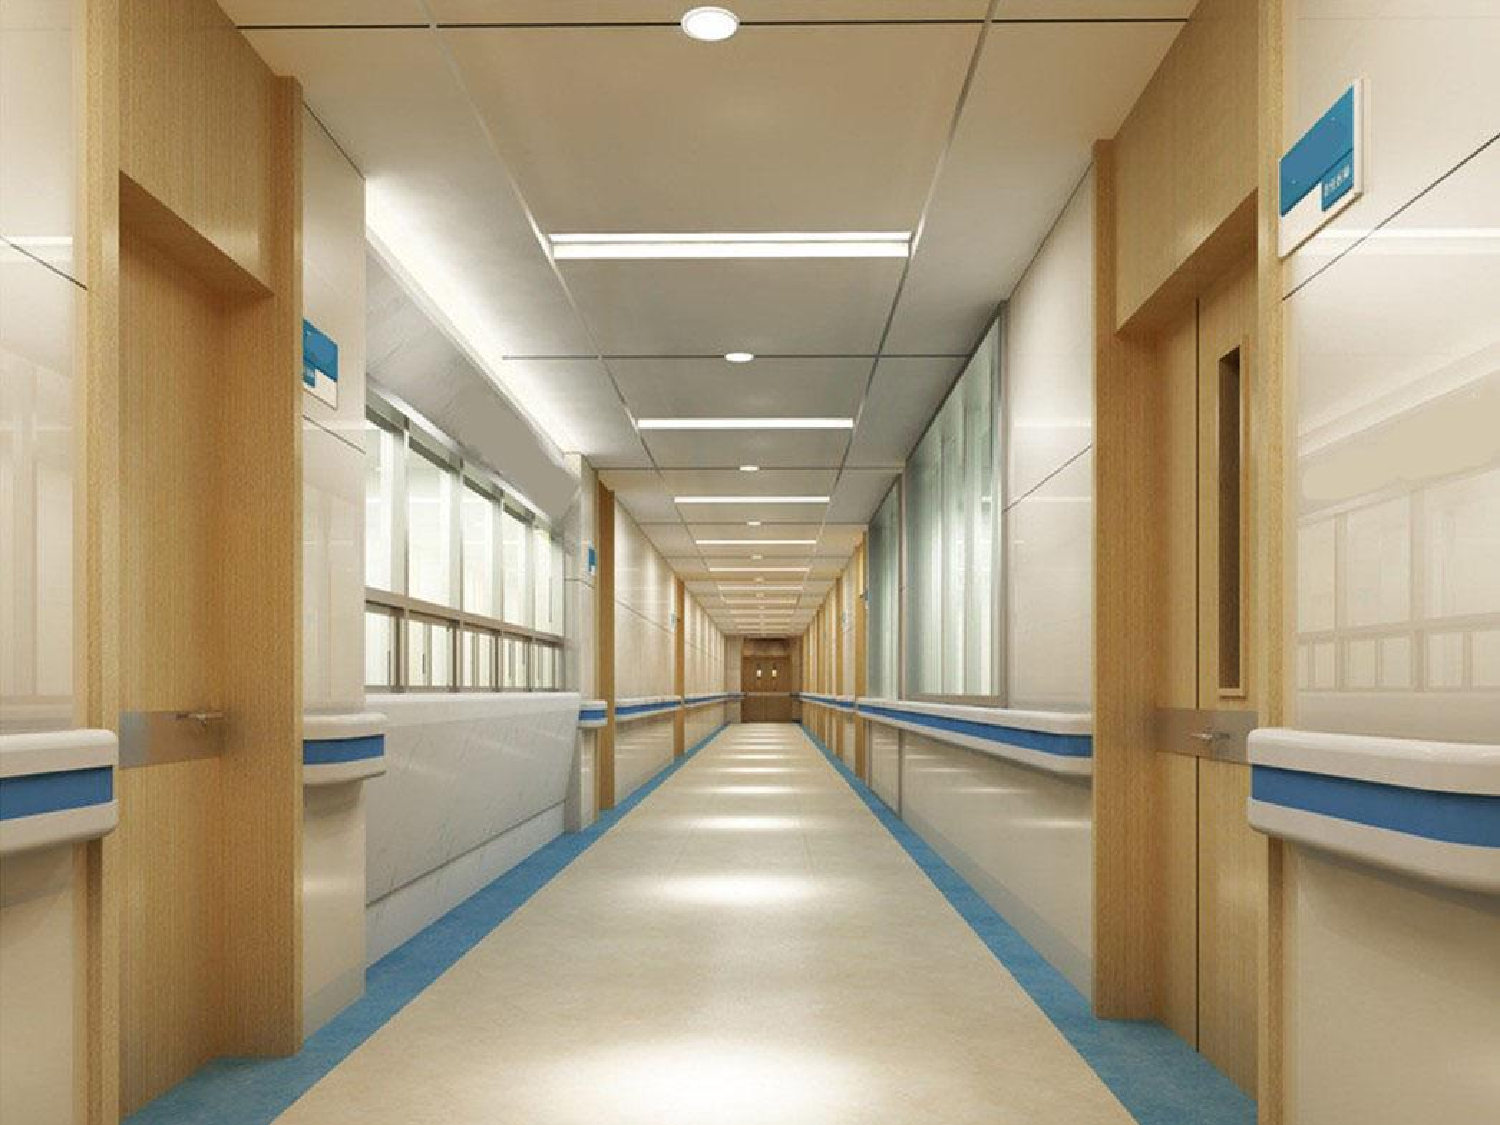
\includegraphics[width=\paperwidth]{images/corridor.pdf}
            };
        \end{tikzpicture}
     \end{frame}
}

%------------------------------------------------

{ % all template changes are local to this group.
    \begin{frame}[plain]
        \begin{tikzpicture}[remember picture,overlay]
            \node[at=(current page.center)] {
                
\includegraphics[width=\paperwidth]{images/moeniafm.pdf}
            };
        \end{tikzpicture}
     \end{frame}
}

%------------------------------------------------

\begin{frame}[fragile]
\frametitle{I'm an Rtist!}
\begin{center}
\ig[height=7cm]{images/blue-rays.pdf}
\end{center}
\end{frame}

%------------------------------------------------

\begin{frame}
\begin{center}
\Huge{\hilit{Me and You}}
\end{center}
\end{frame}

%------------------------------------------------

\begin{frame}
\frametitle{For your significant other}
\begin{center}
\ig[width=11cm]{images/me-and-you.pdf}
\end{center}
\end{frame}

%------------------------------------------------

\begin{frame}[fragile]
\frametitle{For your significant other}

\begin{knitrout}\footnotesize
\definecolor{shadecolor}{rgb}{0.969, 0.969, 0.969}\color{fgcolor}\begin{kframe}
\begin{alltt}
\hlcom{# Number of data points}
\hlstd{n} \hlkwb{<-} \hlnum{100}

\hlcom{# random x-y coordinate values}
\hlkwd{set.seed}\hlstd{(}\hlnum{333}\hlstd{)}
\hlstd{x} \hlkwb{<-} \hlkwd{rnorm}\hlstd{(n)}
\hlstd{y} \hlkwb{<-} \hlkwd{rnorm}\hlstd{(n,} \hlnum{1}\hlstd{,} \hlnum{2}\hlstd{)}

\hlcom{# scatter-plot}
\hlkwd{plot}\hlstd{(x, y,} \hlkwc{type} \hlstd{=} \hlstr{"n"}\hlstd{)}
\hlkwd{text}\hlstd{(x, y,} \hlkwc{labels} \hlstd{=} \hlstr{"me & you"}\hlstd{)}
\end{alltt}
\end{kframe}
\end{knitrout}

\end{frame}

%------------------------------------------------

\begin{frame}[fragile]

\begin{knitrout}
\definecolor{shadecolor}{rgb}{0.969, 0.969, 0.969}\color{fgcolor}
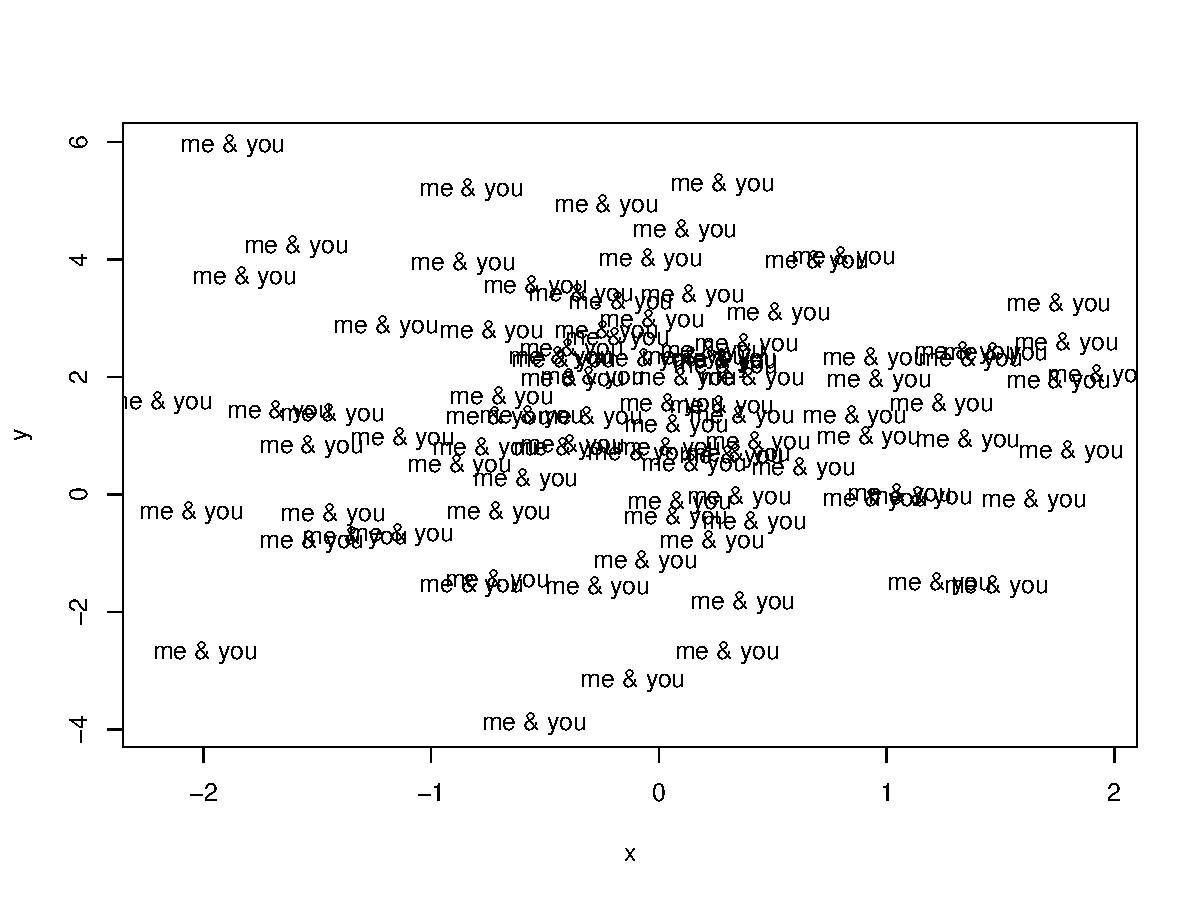
\includegraphics[width=\maxwidth]{figure/me-and-you1-1} 

\end{knitrout}

\end{frame}

%------------------------------------------------

\begin{frame}[fragile]
\frametitle{For your significant other}

\begin{knitrout}\footnotesize
\definecolor{shadecolor}{rgb}{0.969, 0.969, 0.969}\color{fgcolor}\begin{kframe}
\begin{alltt}
\hlcom{# dark gray background}
\hlstd{op} \hlkwb{<-} \hlkwd{par}\hlstd{(}\hlkwc{bg} \hlstd{=} \hlstr{"gray10"}\hlstd{)}

\hlcom{# plot text}
\hlkwd{plot}\hlstd{(x, y,} \hlkwc{type} \hlstd{=} \hlstr{"n"}\hlstd{)}
\hlkwd{text}\hlstd{(x, y,}
     \hlkwc{labels} \hlstd{=} \hlstr{"me & you"}\hlstd{,}
     \hlkwc{col} \hlstd{=} \hlstr{"white"}\hlstd{)}

\hlcom{# reset default graphical parameters}
\hlkwd{par}\hlstd{(op)}
\end{alltt}
\end{kframe}
\end{knitrout}

\end{frame}

%------------------------------------------------

\begin{frame}[fragile]

\begin{knitrout}
\definecolor{shadecolor}{rgb}{0.969, 0.969, 0.969}\color{fgcolor}
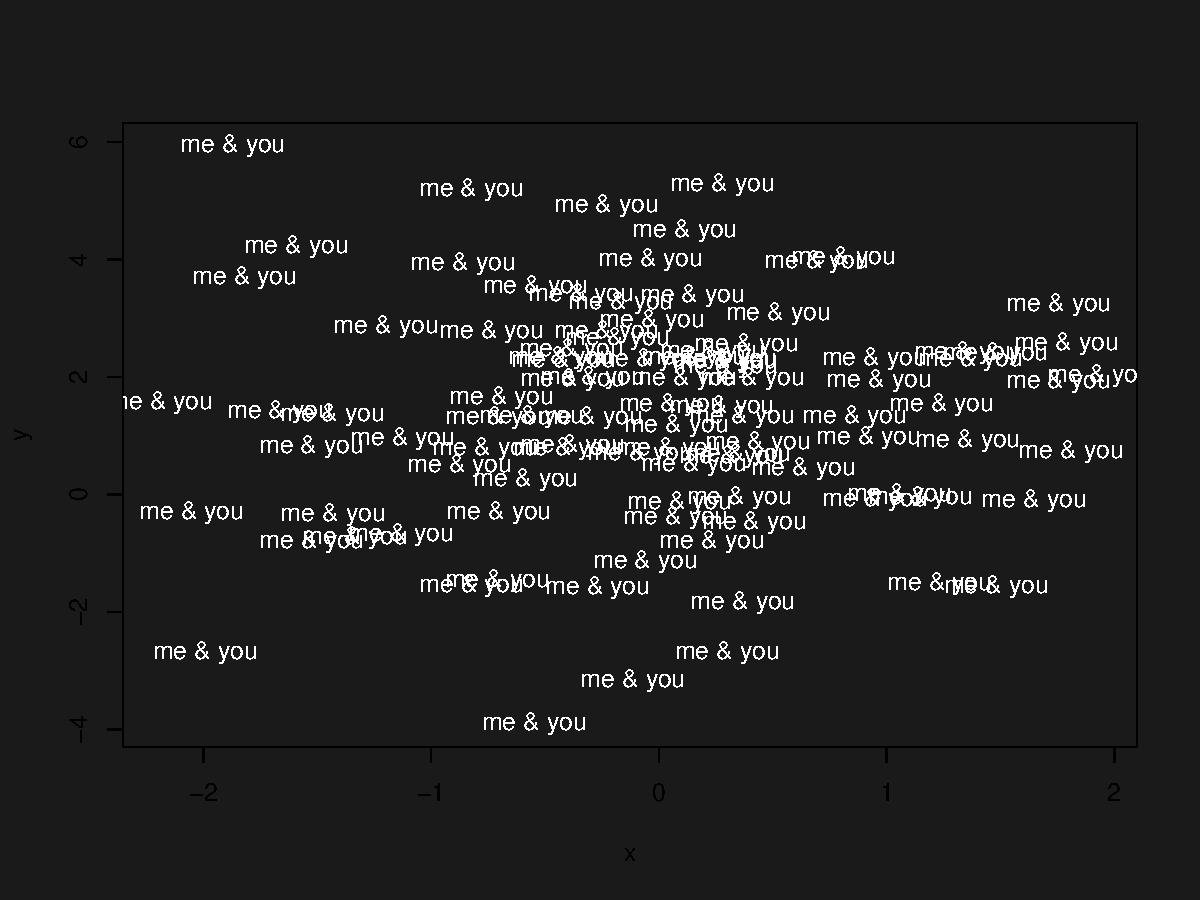
\includegraphics[width=\maxwidth]{figure/me-and-you2-1} 

\end{knitrout}

\end{frame}

%------------------------------------------------

\begin{frame}[fragile]
\frametitle{For your significant other}

\begin{knitrout}\footnotesize
\definecolor{shadecolor}{rgb}{0.969, 0.969, 0.969}\color{fgcolor}\begin{kframe}
\begin{alltt}
\hlcom{# text size and colors}
\hlstd{sizes} \hlkwb{<-} \hlkwd{runif}\hlstd{(n,} \hlnum{0.5}\hlstd{,} \hlnum{3}\hlstd{)}
\hlstd{hues} \hlkwb{<-} \hlkwd{runif}\hlstd{(n,} \hlnum{0.85}\hlstd{,} \hlnum{0.95}\hlstd{)}
\hlstd{alphas} \hlkwb{<-} \hlkwd{runif}\hlstd{(n,} \hlnum{0.1}\hlstd{,} \hlnum{1}\hlstd{)}

\hlcom{# plot}
\hlstd{op} \hlkwb{<-} \hlkwd{par}\hlstd{(}\hlkwc{bg} \hlstd{=} \hlstr{"gray10"}\hlstd{,} \hlkwc{mar} \hlstd{=} \hlkwd{rep}\hlstd{(}\hlnum{0}\hlstd{,} \hlnum{4}\hlstd{))}
\hlkwd{plot}\hlstd{(x, y,} \hlkwc{type} \hlstd{=} \hlstr{"n"}\hlstd{,} \hlkwc{axes} \hlstd{=} \hlnum{FALSE}\hlstd{,} \hlkwc{xlab} \hlstd{=} \hlstr{''}\hlstd{,} \hlkwc{ylab} \hlstd{=} \hlstr{''}\hlstd{)}
\hlkwd{text}\hlstd{(x, y,}
     \hlkwc{labels} \hlstd{=} \hlstr{"me & you"}\hlstd{,}
     \hlkwc{font} \hlstd{=} \hlnum{3}\hlstd{,}
     \hlkwc{col} \hlstd{=} \hlkwd{hsv}\hlstd{(hues,} \hlnum{1}\hlstd{,} \hlnum{1}\hlstd{, alphas),}
     \hlkwc{cex} \hlstd{= sizes)}
\hlkwd{par}\hlstd{(op)}
\end{alltt}
\end{kframe}
\end{knitrout}

\end{frame}

%------------------------------------------------

\begin{frame}[fragile]

\begin{knitrout}
\definecolor{shadecolor}{rgb}{0.969, 0.969, 0.969}\color{fgcolor}

\includegraphics[width=\maxwidth]{figure/me-and-you3-1} 

\end{knitrout}

\end{frame}

%------------------------------------------------

\begin{frame}
\begin{center}
\Huge{\hilit{Humor}}
\end{center}
\end{frame}

%------------------------------------------------

\begin{frame}
\frametitle{Trustworthiness of Beards}
\begin{center}
\ig[width=11cm]{images/beards.pdf}

Designed by Matt McInerney \\
{\scriptsize \url{http://pixelspread.com/images/beards_trust_2.jpg}}
\end{center}
\end{frame}

%------------------------------------------------

\begin{frame}
\frametitle{Trustworthiness of Beards}
\begin{center}
\ig[width=11cm]{images/trustworthy-beards.pdf}
\end{center}
\end{frame}

%------------------------------------------------

\begin{frame}
\frametitle{Trustworthiness of Beards}
\begin{center}
\ig[width=11cm]{images/neutral-beards.pdf}
\end{center}
\end{frame}

%------------------------------------------------

\begin{frame}
\frametitle{Trustworthiness of Beards}
\begin{center}
\ig[width=11cm]{images/dangerous-beards.pdf}
\end{center}
\end{frame}

%------------------------------------------------

\begin{frame}
\begin{center}
\Huge{\hilit{Interesting}}
\end{center}
\end{frame}

%------------------------------------------------

\begin{frame}
\frametitle{Wind Patterns}
\begin{center}
\ig[width=11cm]{images/wind-patterns.pdf}

{\scriptsize \url{http://hint.fm/wind}}
\end{center}
\end{frame}

%------------------------------------------------

\begin{frame}
\frametitle{Similar Diversity (by Steinweber and Koller)}
\begin{center}
\ig[width=11cm]{images/similar-diversity1.pdf}

{\scriptsize \url{http://similardiversity.net/}}
\end{center}
\end{frame}

%------------------------------------------------

\begin{frame}
\frametitle{}
\begin{center}
\ig[height=7cm]{images/similar-diversity3.pdf}
\end{center}
\end{frame}

%------------------------------------------------

\begin{frame}
\frametitle{Similar Diversity (by Steinweber and Koller)}
\begin{center}
\ig[width=11cm]{images/similar-diversity2.pdf}
\end{center}
\end{frame}

%------------------------------------------------

\begin{frame}
\begin{center}
\Huge{\hilit{Playing with Arc Diagrams}}
\end{center}
\end{frame}

%------------------------------------------------

{ % all template changes are local to this group.
    \begin{frame}[plain]
        \begin{tikzpicture}[remember picture,overlay]
            \node[at=(current page.center)] {
                
\includegraphics[width=\paperwidth]{images/star-wars-illustration.pdf}
            };
        \end{tikzpicture}
     \end{frame}
}

%------------------------------------------------

\begin{frame}
\frametitle{Star Wars Original Trilogy}
\begin{center}
\ig[width=11cm]{images/star-wars-trilogy.pdf}
\end{center}
\end{frame}

%------------------------------------------------

\begin{frame}
\begin{center}
\ig[height=9cm]{images/star-wars-movie-script.pdf}
\end{center}
\end{frame}

%------------------------------------------------

\begin{frame}
\begin{center}
\ig[width=11cm]{images/star-wars-arc-diagram1.pdf}
\end{center}
\end{frame}

%------------------------------------------------

\begin{frame}
\begin{center}
\ig[width=11cm]{images/star-wars-arc-diagram2.pdf}
\end{center}
\end{frame}

%------------------------------------------------

\end{document}
